\documentclass[1p]{elsarticle_modified}
%\bibliographystyle{elsarticle-num}

%\usepackage[colorlinks]{hyperref}
%\usepackage{abbrmath_seonhwa} %\Abb, \Ascr, \Acal ,\Abf, \Afrak
\usepackage{amsfonts}
\usepackage{amssymb}
\usepackage{amsmath}
\usepackage{amsthm}
\usepackage{scalefnt}
\usepackage{amsbsy}
\usepackage{kotex}
\usepackage{caption}
\usepackage{subfig}
\usepackage{color}
\usepackage{graphicx}
\usepackage{xcolor} %% white, black, red, green, blue, cyan, magenta, yellow
\usepackage{float}
\usepackage{setspace}
\usepackage{hyperref}

\usepackage{tikz}
\usetikzlibrary{arrows}

\usepackage{multirow}
\usepackage{array} % fixed length table
\usepackage{hhline}

%%%%%%%%%%%%%%%%%%%%%
\makeatletter
\renewcommand*\env@matrix[1][\arraystretch]{%
	\edef\arraystretch{#1}%
	\hskip -\arraycolsep
	\let\@ifnextchar\new@ifnextchar
	\array{*\c@MaxMatrixCols c}}
\makeatother %https://tex.stackexchange.com/questions/14071/how-can-i-increase-the-line-spacing-in-a-matrix
%%%%%%%%%%%%%%%

\usepackage[normalem]{ulem}

\newcommand{\msout}[1]{\ifmmode\text{\sout{\ensuremath{#1}}}\else\sout{#1}\fi}
%SOURCE: \msout is \stkout macro in https://tex.stackexchange.com/questions/20609/strikeout-in-math-mode

\newcommand{\cancel}[1]{
	\ifmmode
	{\color{red}\msout{#1}}
	\else
	{\color{red}\sout{#1}}
	\fi
}

\newcommand{\add}[1]{
	{\color{blue}\uwave{#1}}
}

\newcommand{\replace}[2]{
	\ifmmode
	{\color{red}\msout{#1}}{\color{blue}\uwave{#2}}
	\else
	{\color{red}\sout{#1}}{\color{blue}\uwave{#2}}
	\fi
}

\newcommand{\Sol}{\mathcal{S}} %segment
\newcommand{\D}{D} %diagram
\newcommand{\A}{\mathcal{A}} %arc


%%%%%%%%%%%%%%%%%%%%%%%%%%%%%5 test

\def\sl{\operatorname{\textup{SL}}(2,\Cbb)}
\def\psl{\operatorname{\textup{PSL}}(2,\Cbb)}
\def\quan{\mkern 1mu \triangleright \mkern 1mu}

\theoremstyle{definition}
\newtheorem{thm}{Theorem}[section]
\newtheorem{prop}[thm]{Proposition}
\newtheorem{lem}[thm]{Lemma}
\newtheorem{ques}[thm]{Question}
\newtheorem{cor}[thm]{Corollary}
\newtheorem{defn}[thm]{Definition}
\newtheorem{exam}[thm]{Example}
\newtheorem{rmk}[thm]{Remark}
\newtheorem{alg}[thm]{Algorithm}

\newcommand{\I}{\sqrt{-1}}
\begin{document}

%\begin{frontmatter}
%
%\title{Boundary parabolic representations of knots up to 8 crossings}
%
%%% Group authors per affiliation:
%\author{Yunhi Cho} 
%\address{Department of Mathematics, University of Seoul, Seoul, Korea}
%\ead{yhcho@uos.ac.kr}
%
%
%\author{Seonhwa Kim} %\fnref{s_kim}}
%\address{Center for Geometry and Physics, Institute for Basic Science, Pohang, 37673, Korea}
%\ead{ryeona17@ibs.re.kr}
%
%\author{Hyuk Kim}
%\address{Department of Mathematical Sciences, Seoul National University, Seoul 08826, Korea}
%\ead{hyukkim@snu.ac.kr}
%
%\author{Seokbeom Yoon}
%\address{Department of Mathematical Sciences, Seoul National University, Seoul, 08826,  Korea}
%\ead{sbyoon15@snu.ac.kr}
%
%\begin{abstract}
%We find all boundary parabolic representation of knots up to 8 crossings.
%
%\end{abstract}
%\begin{keyword}
%    \MSC[2010] 57M25 
%\end{keyword}
%
%\end{frontmatter}

%\linenumbers
%\tableofcontents
%
\newcommand\colored[1]{\textcolor{white}{\rule[-0.35ex]{0.8em}{1.4ex}}\kern-0.8em\color{red} #1}%
%\newcommand\colored[1]{\textcolor{white}{ #1}\kern-2.17ex	\textcolor{white}{ #1}\kern-1.81ex	\textcolor{white}{ #1}\kern-2.15ex\color{red}#1	}

{\Large $\underline{12n_{0166}~(K12n_{0166})}$}

\setlength{\tabcolsep}{10pt}
\renewcommand{\arraystretch}{1.6}
\vspace{1cm}\begin{tabular}{m{100pt}>{\centering\arraybackslash}m{274pt}}
\multirow{5}{120pt}{
	\centering
	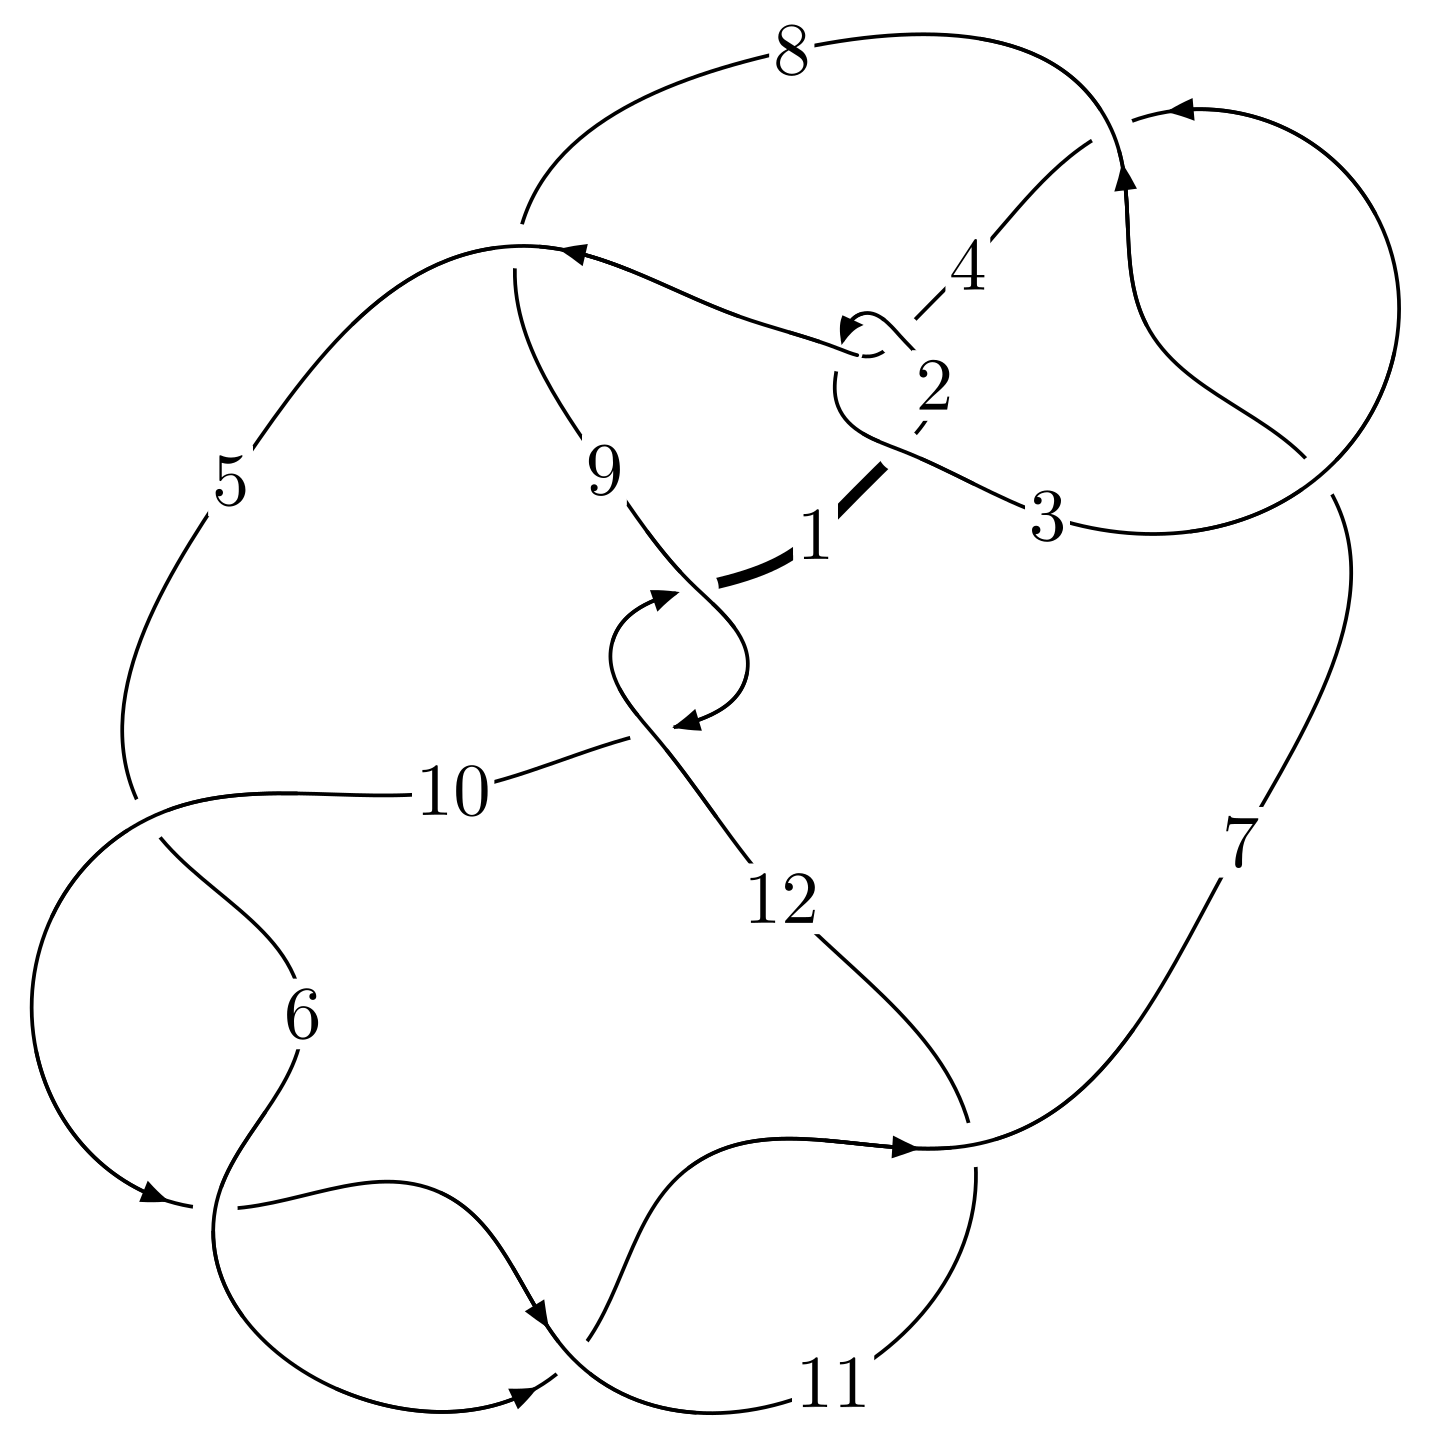
\includegraphics[width=112pt]{../../../GIT/diagram.site/Diagrams/png/2255_12n_0166.png}\\
\ \ \ A knot diagram\footnotemark}&
\allowdisplaybreaks
\textbf{Linearized knot diagam} \\
\cline{2-2}
 &
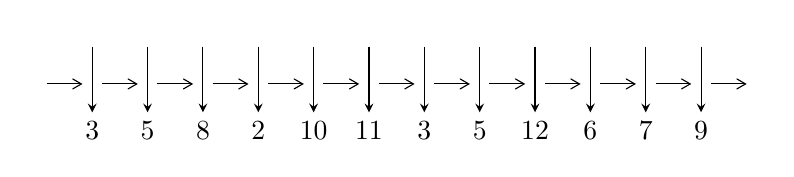
\begin{tikzpicture}[x=20pt, y=17pt]
	% nodes
	\node (C0) at (0, 0) {};
	\node (C1) at (1, 0) {};
	\node (C1U) at (1, +1) {};
	\node (C1D) at (1, -1) {3};

	\node (C2) at (2, 0) {};
	\node (C2U) at (2, +1) {};
	\node (C2D) at (2, -1) {5};

	\node (C3) at (3, 0) {};
	\node (C3U) at (3, +1) {};
	\node (C3D) at (3, -1) {8};

	\node (C4) at (4, 0) {};
	\node (C4U) at (4, +1) {};
	\node (C4D) at (4, -1) {2};

	\node (C5) at (5, 0) {};
	\node (C5U) at (5, +1) {};
	\node (C5D) at (5, -1) {10};

	\node (C6) at (6, 0) {};
	\node (C6U) at (6, +1) {};
	\node (C6D) at (6, -1) {11};

	\node (C7) at (7, 0) {};
	\node (C7U) at (7, +1) {};
	\node (C7D) at (7, -1) {3};

	\node (C8) at (8, 0) {};
	\node (C8U) at (8, +1) {};
	\node (C8D) at (8, -1) {5};

	\node (C9) at (9, 0) {};
	\node (C9U) at (9, +1) {};
	\node (C9D) at (9, -1) {12};

	\node (C10) at (10, 0) {};
	\node (C10U) at (10, +1) {};
	\node (C10D) at (10, -1) {6};

	\node (C11) at (11, 0) {};
	\node (C11U) at (11, +1) {};
	\node (C11D) at (11, -1) {7};

	\node (C12) at (12, 0) {};
	\node (C12U) at (12, +1) {};
	\node (C12D) at (12, -1) {9};
	\node (C13) at (13, 0) {};

	% arrows
	\draw[->,>={angle 60}]
	(C0) edge (C1) (C1) edge (C2) (C2) edge (C3) (C3) edge (C4) (C4) edge (C5) (C5) edge (C6) (C6) edge (C7) (C7) edge (C8) (C8) edge (C9) (C9) edge (C10) (C10) edge (C11) (C11) edge (C12) (C12) edge (C13) ;	\draw[->,>=stealth]
	(C1U) edge (C1D) (C2U) edge (C2D) (C3U) edge (C3D) (C4U) edge (C4D) (C5U) edge (C5D) (C6U) edge (C6D) (C7U) edge (C7D) (C8U) edge (C8D) (C9U) edge (C9D) (C10U) edge (C10D) (C11U) edge (C11D) (C12U) edge (C12D) ;
	\end{tikzpicture} \\
\hhline{~~} \\& 
\textbf{Solving Sequence} \\ \cline{2-2} 
 &
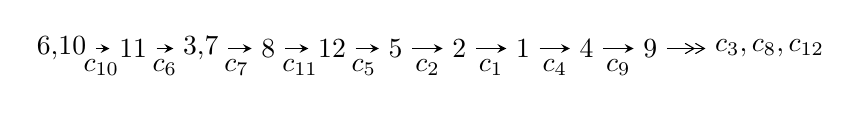
\begin{tikzpicture}[x=23pt, y=7pt]
	% node
	\node (A0) at (-1/8, 0) {6,10};
	\node (A1) at (1, 0) {11};
	\node (A2) at (33/16, 0) {3,7};
	\node (A3) at (25/8, 0) {8};
	\node (A4) at (33/8, 0) {12};
	\node (A5) at (41/8, 0) {5};
	\node (A6) at (49/8, 0) {2};
	\node (A7) at (57/8, 0) {1};
	\node (A8) at (65/8, 0) {4};
	\node (A9) at (73/8, 0) {9};
	\node (C1) at (1/2, -1) {$c_{10}$};
	\node (C2) at (3/2, -1) {$c_{6}$};
	\node (C3) at (21/8, -1) {$c_{7}$};
	\node (C4) at (29/8, -1) {$c_{11}$};
	\node (C5) at (37/8, -1) {$c_{5}$};
	\node (C6) at (45/8, -1) {$c_{2}$};
	\node (C7) at (53/8, -1) {$c_{1}$};
	\node (C8) at (61/8, -1) {$c_{4}$};
	\node (C9) at (69/8, -1) {$c_{9}$};
	\node (A10) at (11, 0) {$c_{3},c_{8},c_{12}$};

	% edge
	\draw[->,>=stealth]	
	(A0) edge (A1) (A1) edge (A2) (A2) edge (A3) (A3) edge (A4) (A4) edge (A5) (A5) edge (A6) (A6) edge (A7) (A7) edge (A8) (A8) edge (A9) ;
	\draw[->>,>={angle 60}]	
	(A9) edge (A10);
\end{tikzpicture} \\ 

\end{tabular} \\

\footnotetext{
The image of knot diagram is generated by the software ``\textbf{Draw programme}" developed by Andrew Bartholomew(\url{http://www.layer8.co.uk/maths/draw/index.htm\#Running-draw}), where we modified some parts for our purpose(\url{https://github.com/CATsTAILs/LinksPainter}).
}\phantom \\ \newline 
\centering \textbf{Ideals for irreducible components\footnotemark of $X_{\text{par}}$} 
 
\begin{align*}
I^u_{1}&=\langle 
u^{25}-14 u^{23}+\cdots+b-1,\;2 u^{25}- u^{24}+\cdots+a-5 u,\;u^{26}-2 u^{25}+\cdots+3 u+1\rangle \\
I^u_{2}&=\langle 
u^4-2 u^2+b+u,\;- u^5+3 u^3+a- u+1,\;u^6+u^5-3 u^4-2 u^3+2 u^2- u-1\rangle \\
\\
\end{align*}
\raggedright * 2 irreducible components of $\dim_{\mathbb{C}}=0$, with total 32 representations.\\
\footnotetext{All coefficients of polynomials are rational numbers. But the coefficients are sometimes approximated in decimal forms when there is not enough margin.}
\newpage
\renewcommand{\arraystretch}{1}
\centering \section*{I. $I^u_{1}= \langle u^{25}-14 u^{23}+\cdots+b-1,\;2 u^{25}- u^{24}+\cdots+a-5 u,\;u^{26}-2 u^{25}+\cdots+3 u+1 \rangle$}
\flushleft \textbf{(i) Arc colorings}\\
\begin{tabular}{m{7pt} m{180pt} m{7pt} m{180pt} }
\flushright $a_{6}=$&$\begin{pmatrix}0\\u\end{pmatrix}$ \\
\flushright $a_{10}=$&$\begin{pmatrix}1\\0\end{pmatrix}$ \\
\flushright $a_{11}=$&$\begin{pmatrix}1\\u^2\end{pmatrix}$ \\
\flushright $a_{3}=$&$\begin{pmatrix}-2 u^{25}+u^{24}+\cdots+9 u^2+5 u\\- u^{25}+14 u^{23}+\cdots+4 u+1\end{pmatrix}$ \\
\flushright $a_{7}=$&$\begin{pmatrix}- u\\- u^3+u\end{pmatrix}$ \\
\flushright $a_{8}=$&$\begin{pmatrix}- u^{10}+5 u^8-8 u^6+5 u^4-3 u^2+1\\- u^{10}+4 u^8-3 u^6-2 u^4- u^2\end{pmatrix}$ \\
\flushright $a_{12}=$&$\begin{pmatrix}- u^2+1\\- u^4+2 u^2\end{pmatrix}$ \\
\flushright $a_{5}=$&$\begin{pmatrix}u\\u\end{pmatrix}$ \\
\flushright $a_{2}=$&$\begin{pmatrix}- u^{25}+u^{24}+\cdots+u-1\\u^{22}-12 u^{20}+\cdots-4 u^3-3 u^2\end{pmatrix}$ \\
\flushright $a_{1}=$&$\begin{pmatrix}u^{10}-5 u^8+8 u^6-5 u^4+3 u^2-1\\u^{12}-6 u^{10}+12 u^8-8 u^6+u^4-2 u^2\end{pmatrix}$ \\
\flushright $a_{4}=$&$\begin{pmatrix}u^{24}-13 u^{22}+\cdots- u-1\\u^{25}-14 u^{23}+\cdots-3 u-1\end{pmatrix}$ \\
\flushright $a_{9}=$&$\begin{pmatrix}- u^6+3 u^4-2 u^2+1\\- u^8+4 u^6-4 u^4\end{pmatrix}$\\&\end{tabular}
\flushleft \textbf{(ii) Obstruction class $= -1$}\\~\\
\flushleft \textbf{(iii) Cusp Shapes $= -4 u^{25}+5 u^{24}+51 u^{23}-62 u^{22}-269 u^{21}+312 u^{20}+760 u^{19}-813 u^{18}-1264 u^{17}+1176 u^{16}+1341 u^{15}-1013 u^{14}-1049 u^{13}+682 u^{12}+692 u^{11}-399 u^{10}-430 u^9+65 u^8+311 u^7-6 u^6-115 u^5-18 u^4+50 u^3+9 u^2-6 u-18$}\\~\\
\newpage\renewcommand{\arraystretch}{1}
\flushleft \textbf{(iv) u-Polynomials at the component}\newline \\
\begin{tabular}{m{50pt}|m{274pt}}
Crossings & \hspace{64pt}u-Polynomials at each crossing \\
\hline $$\begin{aligned}c_{1}\end{aligned}$$&$\begin{aligned}
&u^{26}+37 u^{25}+\cdots+76 u+1
\end{aligned}$\\
\hline $$\begin{aligned}c_{2},c_{4}\end{aligned}$$&$\begin{aligned}
&u^{26}-7 u^{25}+\cdots-2 u-1
\end{aligned}$\\
\hline $$\begin{aligned}c_{3},c_{7}\end{aligned}$$&$\begin{aligned}
&u^{26}- u^{25}+\cdots-128 u-64
\end{aligned}$\\
\hline $$\begin{aligned}c_{5},c_{6},c_{10}\\c_{11}\end{aligned}$$&$\begin{aligned}
&u^{26}-2 u^{25}+\cdots+3 u+1
\end{aligned}$\\
\hline $$\begin{aligned}c_{8}\end{aligned}$$&$\begin{aligned}
&u^{26}+2 u^{25}+\cdots+3 u+1
\end{aligned}$\\
\hline $$\begin{aligned}c_{9},c_{12}\end{aligned}$$&$\begin{aligned}
&u^{26}-6 u^{25}+\cdots-21 u-9
\end{aligned}$\\
\hline
\end{tabular}\\~\\
\newpage\renewcommand{\arraystretch}{1}
\flushleft \textbf{(v) Riley Polynomials at the component}\newline \\
\begin{tabular}{m{50pt}|m{274pt}}
Crossings & \hspace{64pt}Riley Polynomials at each crossing \\
\hline $$\begin{aligned}c_{1}\end{aligned}$$&$\begin{aligned}
&y^{26}-89 y^{25}+\cdots-2892 y+1
\end{aligned}$\\
\hline $$\begin{aligned}c_{2},c_{4}\end{aligned}$$&$\begin{aligned}
&y^{26}-37 y^{25}+\cdots-76 y+1
\end{aligned}$\\
\hline $$\begin{aligned}c_{3},c_{7}\end{aligned}$$&$\begin{aligned}
&y^{26}-39 y^{25}+\cdots-12288 y+4096
\end{aligned}$\\
\hline $$\begin{aligned}c_{5},c_{6},c_{10}\\c_{11}\end{aligned}$$&$\begin{aligned}
&y^{26}-30 y^{25}+\cdots-11 y+1
\end{aligned}$\\
\hline $$\begin{aligned}c_{8}\end{aligned}$$&$\begin{aligned}
&y^{26}-54 y^{25}+\cdots-11 y+1
\end{aligned}$\\
\hline $$\begin{aligned}c_{9},c_{12}\end{aligned}$$&$\begin{aligned}
&y^{26}+6 y^{25}+\cdots-531 y+81
\end{aligned}$\\
\hline
\end{tabular}\\~\\
\newpage\flushleft \textbf{(vi) Complex Volumes and Cusp Shapes}
$$\begin{array}{c|c|c}  
\text{Solutions to }I^u_{1}& \I (\text{vol} + \sqrt{-1}CS) & \text{Cusp shape}\\
 \hline 
\begin{aligned}
u &= -0.681707 + 0.582351 I \\
a &= -0.132311 + 0.107455 I \\
b &= -1.80048 - 0.98897 I\end{aligned}
 & -10.93830 + 7.21103 I & -16.0759 - 5.4438 I \\ \hline\begin{aligned}
u &= -0.681707 - 0.582351 I \\
a &= -0.132311 - 0.107455 I \\
b &= -1.80048 + 0.98897 I\end{aligned}
 & -10.93830 - 7.21103 I & -16.0759 + 5.4438 I \\ \hline\begin{aligned}
u &= \phantom{-}1.175060 + 0.078346 I \\
a &= \phantom{-}0.222046 + 0.015295 I \\
b &= \phantom{-}1.71753 - 0.10327 I\end{aligned}
 & -14.2898 + 0.0080 I & -18.3523 + 0.3239 I \\ \hline\begin{aligned}
u &= \phantom{-}1.175060 - 0.078346 I \\
a &= \phantom{-}0.222046 - 0.015295 I \\
b &= \phantom{-}1.71753 + 0.10327 I\end{aligned}
 & -14.2898 - 0.0080 I & -18.3523 - 0.3239 I \\ \hline\begin{aligned}
u &= -0.615423 + 0.435220 I \\
a &= \phantom{-}0.006046 + 0.650453 I \\
b &= \phantom{-}1.43706 + 0.60644 I\end{aligned}
 & -1.64268 + 3.44770 I & -15.9366 - 6.5929 I \\ \hline\begin{aligned}
u &= -0.615423 - 0.435220 I \\
a &= \phantom{-}0.006046 - 0.650453 I \\
b &= \phantom{-}1.43706 - 0.60644 I\end{aligned}
 & -1.64268 - 3.44770 I & -15.9366 + 6.5929 I \\ \hline\begin{aligned}
u &= \phantom{-}0.492369 + 0.545154 I \\
a &= \phantom{-}0.033687 + 0.462693 I \\
b &= \phantom{-}0.322628 + 0.025417 I\end{aligned}
 & \phantom{-}2.35945 - 1.88336 I & -5.73263 + 3.81073 I \\ \hline\begin{aligned}
u &= \phantom{-}0.492369 - 0.545154 I \\
a &= \phantom{-}0.033687 - 0.462693 I \\
b &= \phantom{-}0.322628 - 0.025417 I\end{aligned}
 & \phantom{-}2.35945 + 1.88336 I & -5.73263 - 3.81073 I \\ \hline\begin{aligned}
u &= -0.265310 + 0.672765 I \\
a &= \phantom{-}0.80138 + 1.96514 I \\
b &= \phantom{-}0.117100 - 0.374073 I\end{aligned}
 & -9.70379 - 2.98173 I & -13.78370 + 0.17341 I \\ \hline\begin{aligned}
u &= -0.265310 - 0.672765 I \\
a &= \phantom{-}0.80138 - 1.96514 I \\
b &= \phantom{-}0.117100 + 0.374073 I\end{aligned}
 & -9.70379 + 2.98173 I & -13.78370 - 0.17341 I\\
 \hline 
 \end{array}$$\newpage$$\begin{array}{c|c|c}  
\text{Solutions to }I^u_{1}& \I (\text{vol} + \sqrt{-1}CS) & \text{Cusp shape}\\
 \hline 
\begin{aligned}
u &= \phantom{-}0.589835 + 0.287549 I \\
a &= \phantom{-}0.399854 - 1.018310 I \\
b &= -1.126490 + 0.098071 I\end{aligned}
 & -2.66891 - 0.88385 I & -16.9206 + 6.0063 I \\ \hline\begin{aligned}
u &= \phantom{-}0.589835 - 0.287549 I \\
a &= \phantom{-}0.399854 + 1.018310 I \\
b &= -1.126490 - 0.098071 I\end{aligned}
 & -2.66891 + 0.88385 I & -16.9206 - 6.0063 I \\ \hline\begin{aligned}
u &= -0.277498 + 0.391559 I \\
a &= -0.71760 - 1.38397 I \\
b &= -0.619638 + 0.253799 I\end{aligned}
 & -0.683753 - 0.414385 I & -12.43905 - 0.47517 I \\ \hline\begin{aligned}
u &= -0.277498 - 0.391559 I \\
a &= -0.71760 + 1.38397 I \\
b &= -0.619638 - 0.253799 I\end{aligned}
 & -0.683753 + 0.414385 I & -12.43905 + 0.47517 I \\ \hline\begin{aligned}
u &= \phantom{-}1.52883 + 0.05644 I \\
a &= \phantom{-}0.949715 - 0.290539 I \\
b &= \phantom{-}0.830011 + 0.081100 I\end{aligned}
 & -6.94574 - 0.62089 I & -15.5634 - 0.9743 I \\ \hline\begin{aligned}
u &= \phantom{-}1.52883 - 0.05644 I \\
a &= \phantom{-}0.949715 + 0.290539 I \\
b &= \phantom{-}0.830011 - 0.081100 I\end{aligned}
 & -6.94574 + 0.62089 I & -15.5634 + 0.9743 I \\ \hline\begin{aligned}
u &= -1.52725 + 0.15077 I \\
a &= -0.741655 - 0.245504 I \\
b &= -1.002680 - 0.376527 I\end{aligned}
 & -4.34854 + 4.33683 I & -10.06939 - 2.72465 I \\ \hline\begin{aligned}
u &= -1.52725 - 0.15077 I \\
a &= -0.741655 + 0.245504 I \\
b &= -1.002680 + 0.376527 I\end{aligned}
 & -4.34854 - 4.33683 I & -10.06939 + 2.72465 I \\ \hline\begin{aligned}
u &= -1.57781 + 0.08698 I \\
a &= \phantom{-}2.47671 + 0.53175 I \\
b &= \phantom{-}3.33781 + 0.79397 I\end{aligned}
 & -10.09930 + 2.28663 I & -19.0760 - 2.3439 I \\ \hline\begin{aligned}
u &= -1.57781 - 0.08698 I \\
a &= \phantom{-}2.47671 - 0.53175 I \\
b &= \phantom{-}3.33781 - 0.79397 I\end{aligned}
 & -10.09930 - 2.28663 I & -19.0760 + 2.3439 I\\
 \hline 
 \end{array}$$\newpage$$\begin{array}{c|c|c}  
\text{Solutions to }I^u_{1}& \I (\text{vol} + \sqrt{-1}CS) & \text{Cusp shape}\\
 \hline 
\begin{aligned}
u &= \phantom{-}1.57863 + 0.12294 I \\
a &= -2.06274 + 1.32680 I \\
b &= -2.70573 + 0.88516 I\end{aligned}
 & -9.08260 - 5.47988 I & -18.5451 + 4.2333 I \\ \hline\begin{aligned}
u &= \phantom{-}1.57863 - 0.12294 I \\
a &= -2.06274 - 1.32680 I \\
b &= -2.70573 - 0.88516 I\end{aligned}
 & -9.08260 + 5.47988 I & -18.5451 - 4.2333 I \\ \hline\begin{aligned}
u &= \phantom{-}1.59730 + 0.17727 I \\
a &= \phantom{-}2.38789 - 2.06908 I \\
b &= \phantom{-}3.52206 - 2.02315 I\end{aligned}
 & -18.6017 - 10.0445 I & -18.6964 + 4.4096 I \\ \hline\begin{aligned}
u &= \phantom{-}1.59730 - 0.17727 I \\
a &= \phantom{-}2.38789 + 2.06908 I \\
b &= \phantom{-}3.52206 + 2.02315 I\end{aligned}
 & -18.6017 + 10.0445 I & -18.6964 - 4.4096 I \\ \hline\begin{aligned}
u &= -0.383361\phantom{ +0.000000I} \\
a &= -0.709996\phantom{ +0.000000I} \\
b &= -0.351806\phantom{ +0.000000I}\end{aligned}
 & -0.582197\phantom{ +0.000000I} & -16.9580\phantom{ +0.000000I} \\ \hline\begin{aligned}
u &= -1.65067\phantom{ +0.000000I} \\
a &= -3.53607\phantom{ +0.000000I} \\
b &= -4.70658\phantom{ +0.000000I}\end{aligned}
 & \phantom{-}15.9598\phantom{ +0.000000I} & -20.6600\phantom{ +0.000000I}\\
 \hline 
 \end{array}$$\newpage\newpage\renewcommand{\arraystretch}{1}
\centering \section*{II. $I^u_{2}= \langle u^4-2 u^2+b+u,\;- u^5+3 u^3+a- u+1,\;u^6+u^5-3 u^4-2 u^3+2 u^2- u-1 \rangle$}
\flushleft \textbf{(i) Arc colorings}\\
\begin{tabular}{m{7pt} m{180pt} m{7pt} m{180pt} }
\flushright $a_{6}=$&$\begin{pmatrix}0\\u\end{pmatrix}$ \\
\flushright $a_{10}=$&$\begin{pmatrix}1\\0\end{pmatrix}$ \\
\flushright $a_{11}=$&$\begin{pmatrix}1\\u^2\end{pmatrix}$ \\
\flushright $a_{3}=$&$\begin{pmatrix}u^5-3 u^3+u-1\\- u^4+2 u^2- u\end{pmatrix}$ \\
\flushright $a_{7}=$&$\begin{pmatrix}- u\\- u^3+u\end{pmatrix}$ \\
\flushright $a_{8}=$&$\begin{pmatrix}- u\\- u^3+u\end{pmatrix}$ \\
\flushright $a_{12}=$&$\begin{pmatrix}- u^2+1\\- u^4+2 u^2\end{pmatrix}$ \\
\flushright $a_{5}=$&$\begin{pmatrix}u\\u\end{pmatrix}$ \\
\flushright $a_{2}=$&$\begin{pmatrix}u^5-3 u^3-1\\- u^4+2 u^2-2 u\end{pmatrix}$ \\
\flushright $a_{1}=$&$\begin{pmatrix}- u\\- u\end{pmatrix}$ \\
\flushright $a_{4}=$&$\begin{pmatrix}u^5-3 u^3+u-1\\- u^4+2 u^2- u\end{pmatrix}$ \\
\flushright $a_{9}=$&$\begin{pmatrix}u^5-2 u^3- u\\u^5-3 u^3+u\end{pmatrix}$\\&\end{tabular}
\flushleft \textbf{(ii) Obstruction class $= 1$}\\~\\
\flushleft \textbf{(iii) Cusp Shapes $= -3 u^5- u^4+6 u^3+u^2+2 u-14$}\\~\\
\newpage\renewcommand{\arraystretch}{1}
\flushleft \textbf{(iv) u-Polynomials at the component}\newline \\
\begin{tabular}{m{50pt}|m{274pt}}
Crossings & \hspace{64pt}u-Polynomials at each crossing \\
\hline $$\begin{aligned}c_{1},c_{2}\end{aligned}$$&$\begin{aligned}
&(u-1)^6
\end{aligned}$\\
\hline $$\begin{aligned}c_{3},c_{7}\end{aligned}$$&$\begin{aligned}
&u^6
\end{aligned}$\\
\hline $$\begin{aligned}c_{4}\end{aligned}$$&$\begin{aligned}
&(u+1)^6
\end{aligned}$\\
\hline $$\begin{aligned}c_{5},c_{6}\end{aligned}$$&$\begin{aligned}
&u^6- u^5-3 u^4+2 u^3+2 u^2+u-1
\end{aligned}$\\
\hline $$\begin{aligned}c_{8},c_{12}\end{aligned}$$&$\begin{aligned}
&u^6- u^5+3 u^4-2 u^3+2 u^2- u-1
\end{aligned}$\\
\hline $$\begin{aligned}c_{9}\end{aligned}$$&$\begin{aligned}
&u^6+u^5+3 u^4+2 u^3+2 u^2+u-1
\end{aligned}$\\
\hline $$\begin{aligned}c_{10},c_{11}\end{aligned}$$&$\begin{aligned}
&u^6+u^5-3 u^4-2 u^3+2 u^2- u-1
\end{aligned}$\\
\hline
\end{tabular}\\~\\
\newpage\renewcommand{\arraystretch}{1}
\flushleft \textbf{(v) Riley Polynomials at the component}\newline \\
\begin{tabular}{m{50pt}|m{274pt}}
Crossings & \hspace{64pt}Riley Polynomials at each crossing \\
\hline $$\begin{aligned}c_{1},c_{2},c_{4}\end{aligned}$$&$\begin{aligned}
&(y-1)^6
\end{aligned}$\\
\hline $$\begin{aligned}c_{3},c_{7}\end{aligned}$$&$\begin{aligned}
&y^6
\end{aligned}$\\
\hline $$\begin{aligned}c_{5},c_{6},c_{10}\\c_{11}\end{aligned}$$&$\begin{aligned}
&y^6-7 y^5+17 y^4-16 y^3+6 y^2-5 y+1
\end{aligned}$\\
\hline $$\begin{aligned}c_{8},c_{9},c_{12}\end{aligned}$$&$\begin{aligned}
&y^6+5 y^5+9 y^4+4 y^3-6 y^2-5 y+1
\end{aligned}$\\
\hline
\end{tabular}\\~\\
\newpage\flushleft \textbf{(vi) Complex Volumes and Cusp Shapes}
$$\begin{array}{c|c|c}  
\text{Solutions to }I^u_{2}& \I (\text{vol} + \sqrt{-1}CS) & \text{Cusp shape}\\
 \hline 
\begin{aligned}
u &= \phantom{-}0.493180 + 0.575288 I \\
a &= \phantom{-}0.504580 - 0.342767 I \\
b &= -0.354346 + 0.659157 I\end{aligned}
 & \phantom{-}1.31531 - 1.97241 I & -14.7121 + 3.8836 I \\ \hline\begin{aligned}
u &= \phantom{-}0.493180 - 0.575288 I \\
a &= \phantom{-}0.504580 + 0.342767 I \\
b &= -0.354346 - 0.659157 I\end{aligned}
 & \phantom{-}1.31531 + 1.97241 I & -14.7121 - 3.8836 I \\ \hline\begin{aligned}
u &= -0.483672\phantom{ +0.000000I} \\
a &= -1.17069\phantom{ +0.000000I} \\
b &= \phantom{-}0.896823\phantom{ +0.000000I}\end{aligned}
 & -2.38379\phantom{ +0.000000I} & -15.3880\phantom{ +0.000000I} \\ \hline\begin{aligned}
u &= -1.52087 + 0.16310 I \\
a &= \phantom{-}0.462019 + 1.043570 I \\
b &= \phantom{-}1.11206 + 1.11328 I\end{aligned}
 & -5.34051 + 4.59213 I & -18.4963 - 3.9250 I \\ \hline\begin{aligned}
u &= -1.52087 - 0.16310 I \\
a &= \phantom{-}0.462019 - 1.043570 I \\
b &= \phantom{-}1.11206 - 1.11328 I\end{aligned}
 & -5.34051 - 4.59213 I & -18.4963 + 3.9250 I \\ \hline\begin{aligned}
u &= \phantom{-}1.53904\phantom{ +0.000000I} \\
a &= -1.76250\phantom{ +0.000000I} \\
b &= -2.41226\phantom{ +0.000000I}\end{aligned}
 & -9.30502\phantom{ +0.000000I} & -18.1960\phantom{ +0.000000I}\\
 \hline 
 \end{array}$$\newpage
\newpage\renewcommand{\arraystretch}{1}
\centering \section*{ III. u-Polynomials}
\begin{tabular}{m{50pt}|m{274pt}}
Crossings & \hspace{64pt}u-Polynomials at each crossing \\
\hline $$\begin{aligned}c_{1}\end{aligned}$$&$\begin{aligned}
&((u-1)^6)(u^{26}+37 u^{25}+\cdots+76 u+1)
\end{aligned}$\\
\hline $$\begin{aligned}c_{2}\end{aligned}$$&$\begin{aligned}
&((u-1)^6)(u^{26}-7 u^{25}+\cdots-2 u-1)
\end{aligned}$\\
\hline $$\begin{aligned}c_{3},c_{7}\end{aligned}$$&$\begin{aligned}
&u^6(u^{26}- u^{25}+\cdots-128 u-64)
\end{aligned}$\\
\hline $$\begin{aligned}c_{4}\end{aligned}$$&$\begin{aligned}
&((u+1)^6)(u^{26}-7 u^{25}+\cdots-2 u-1)
\end{aligned}$\\
\hline $$\begin{aligned}c_{5},c_{6}\end{aligned}$$&$\begin{aligned}
&(u^6- u^5-3 u^4+2 u^3+2 u^2+u-1)(u^{26}-2 u^{25}+\cdots+3 u+1)
\end{aligned}$\\
\hline $$\begin{aligned}c_{8}\end{aligned}$$&$\begin{aligned}
&(u^6- u^5+3 u^4-2 u^3+2 u^2- u-1)(u^{26}+2 u^{25}+\cdots+3 u+1)
\end{aligned}$\\
\hline $$\begin{aligned}c_{9}\end{aligned}$$&$\begin{aligned}
&(u^6+u^5+3 u^4+2 u^3+2 u^2+u-1)(u^{26}-6 u^{25}+\cdots-21 u-9)
\end{aligned}$\\
\hline $$\begin{aligned}c_{10},c_{11}\end{aligned}$$&$\begin{aligned}
&(u^6+u^5-3 u^4-2 u^3+2 u^2- u-1)(u^{26}-2 u^{25}+\cdots+3 u+1)
\end{aligned}$\\
\hline $$\begin{aligned}c_{12}\end{aligned}$$&$\begin{aligned}
&(u^6- u^5+3 u^4-2 u^3+2 u^2- u-1)(u^{26}-6 u^{25}+\cdots-21 u-9)
\end{aligned}$\\
\hline
\end{tabular}\newpage\renewcommand{\arraystretch}{1}
\centering \section*{ IV. Riley Polynomials}
\begin{tabular}{m{50pt}|m{274pt}}
Crossings & \hspace{64pt}Riley Polynomials at each crossing \\
\hline $$\begin{aligned}c_{1}\end{aligned}$$&$\begin{aligned}
&((y-1)^6)(y^{26}-89 y^{25}+\cdots-2892 y+1)
\end{aligned}$\\
\hline $$\begin{aligned}c_{2},c_{4}\end{aligned}$$&$\begin{aligned}
&((y-1)^6)(y^{26}-37 y^{25}+\cdots-76 y+1)
\end{aligned}$\\
\hline $$\begin{aligned}c_{3},c_{7}\end{aligned}$$&$\begin{aligned}
&y^6(y^{26}-39 y^{25}+\cdots-12288 y+4096)
\end{aligned}$\\
\hline $$\begin{aligned}c_{5},c_{6},c_{10}\\c_{11}\end{aligned}$$&$\begin{aligned}
&(y^6-7 y^5+\cdots-5 y+1)(y^{26}-30 y^{25}+\cdots-11 y+1)
\end{aligned}$\\
\hline $$\begin{aligned}c_{8}\end{aligned}$$&$\begin{aligned}
&(y^6+5 y^5+\cdots-5 y+1)(y^{26}-54 y^{25}+\cdots-11 y+1)
\end{aligned}$\\
\hline $$\begin{aligned}c_{9},c_{12}\end{aligned}$$&$\begin{aligned}
&(y^6+5 y^5+\cdots-5 y+1)(y^{26}+6 y^{25}+\cdots-531 y+81)
\end{aligned}$\\
\hline
\end{tabular}
\vskip 2pc
\end{document}